\documentclass[12pt]{article}


\usepackage{color}
\usepackage{ulem}
\usepackage{graphicx}
\usepackage{mathtools}
\usepackage{authblk} 
\usepackage{epstopdf}
\usepackage{float}
\usepackage{epstopdf}
\usepackage{float}
\usepackage{lineno}
\usepackage{natbib}
\usepackage{fancyhdr}
\usepackage{amsmath}
\usepackage{listings}
\usepackage{setspace}
\usepackage{gensymb} 
\usepackage{indentfirst}
\usepackage{float}
%\usepackage[parfill]{parskip}

\usepackage[margin=1in]{geometry}

\pagestyle{fancy}

\fancyhead{}
\fancyfoot{}
\fancyhead[CO,CE]{\textit{O. Banerjee / High Energy Neutrinos from Gamma Ray Bursts}}
\fancyfoot[CO,CE]{\thepage}


\begin{document}

%%%%%%%%%%%%%%%%%%%%%%%%%%%%%%%%%%%%%%%%%%%%%%%%%%%%%%%%%%%%%
%%%%%%%%%%%%%%%%%%%%%%%%%%%%%%%%%%%%%%%%%%%%%%%%%%%%%%%%%%%%%
%%%%%%%%%%%%%%%%%%%%%%%%%%%%%%%%%%%%%%%%%%%%%%%%%%%%%%%%%%%%%
\title{\textbf{\Large{High Energy Neutrinos from Gamma Ray Bursts:}}\\ {\Large Theoretical Predictions, Experimental Searches, \\ and Prospects for Detection}}

\author{Oindree Banerjee \\
\medskip
PhD Candidacy Written Examination\\
Department of Physics\\
The Ohio State University\\
Advisor: Prof. Amy Connolly}

%\linenumbers
\maketitle
\begin{abstract}
Gamma-ray bursts (GRBs) are the most luminous transient events in the observed Universe. However, there is no direct observational evidence for what exactly drives a GRB. The most widely accepted model for these cosmic events is the fireball model where it is thought that a substantial fraction of the kinetic energy of the source is converted to gamma-radiation by shock accelerated electrons emitting synchrotron and inverse-Compton radiation. Acceleration of protons in the gamma-ray emitting region of the GRB has been hypothesized as well. In this hadronic acceleration model, it is predicted that protons may interact with gamma-ray photons to produce a burst of neutrinos at energy $\sim 10^{14} \, \mathrm{eV}$ during prompt emission and energy $\sim 10^{18} \, \mathrm{eV}$ during afterglow emission. Several experimental searches for these high energy neutrinos have been conducted and no GRB neutrinos have yet been found. The analytical prediction for neutrino flux has been replaced with a more thorough numerical prediction for neutrino flux. The neutron model of GRBs, where only neutrons are able to escape the GRB and reach Earth as cosmic rays, has been ruled out by the experimental work of IceCube and ANTARES. Upgraded versions of current experiments such as IceCube, ANTARES, ANITA and ARA, as well as new experiments such as KM3NeT, are preparing to probe and further constrain the fireball paradigm of GRB neutrino production. \end{abstract}
\newpage
\tableofcontents

\newpage
\begin{doublespace}

%------------------------------------------------------------------------
%-----------------------NEW SECTION----------------------------
%------------------------------------------------------------------------

\section{Introduction}

Gamma-ray bursts (GRBs) are the most luminous transient events in the observed Universe. They were first discovered in 1967 by the Vela satellites flown by the U.S. Department of Defense to look for any possible breach of the Nuclear Test Ban Treaty. These intense bursts of gamma-ray radiation continue to intrigue and puzzle scientists to this day; however, research in the past decades have revealed much about them including that they are extragalactic in origin, isotropically distributed and that they come in at least two populations depending on whether they last for a long ($t_{GRB} > 2 \, \mathrm{s}$) or short ($t_{GRB} < 2 \, \mathrm{s}$) time. Gamma-ray luminosities of GRBs are of the order $10^{52} \, \mathrm{erg \, s^{-1}}$ which can be compared to the $10^{33} \, \mathrm{erg \, s^{-1}}$ emitted by our Sun, $10^{41} \, \mathrm{erg \, s^{-1}}$ by a supernova and $10^{45} \, \mathrm{erg \, s^{-1}}$ by a whole galaxy. GRBs can last for less than one second to several hundreds of seconds (5400 second long GRB reported in \cite{longhardgrb}) and while they last, they can outshine an entire galaxy \cite{Meszaros,MBthesis}. It is thought that long bursts are associated with the collapse of massive stars or hypernovae and that short bursts are associated with mergers of binaries composed of neutron star--neutron star or neutron star--black hole \cite{Meszaros}. However, there is no direct observational evidence for what exactly drives a GRB. \par
From the available gamma-ray observations alone, GRB theorists have hypothesized that regardless of the nature of the underlying source or progenitor, GRBs are produced by the dissipation of the kinetic energy of a relativistically expanding fireball. They have suggested that protons may be Fermi accelerated in this dissipation region to energies $> 10^{20} \, \mathrm{eV}$. Theorized interactions between fireball gamma-ray photons of energy $\sim 1 \, \mathrm{MeV}$ and accelerated protons of energy $\sim 10^{15} \, \mathrm{eV}$ may lead to photo-meson production of pions that may decay resulting in an accompanying burst of $\sim 10^{14} \, \mathrm{eV}$ neutrinos (Waxman \textit{et al.} \cite{Waxmanreview,firstcalc}). The detection of GRB neutrinos would provide unambiguous proof for hadronic acceleration in these cosmic explosions and could also explain the origin of the cosmic ray flux at ultra-high energies.\par
In this paper, we discuss theoretical predictions, experimental searches and prospects for detection of high energy neutrinos from GRBs. Here, high energy is defined as $\sim 10^{11} \, \mathrm{eV}$ and above. This includes the ultra-high energy (UHE) regime which is energy above $10^{17} \, \mathrm{eV}$. We discuss the fireball model and the early predictions made for neutrino fluences in Section 2 of this paper. In Section 3 of this paper, we give a brief overview of different neutrino experiments and how they complement one another. In Section 4 we discuss experimental searches for high energy neutrinos from GRBs and their results. In Section 5, we write about the prospects for detection of high energy neutrinos in the future.

%------------------------------------------------------------------------
%-----------------------NEW SECTION----------------------------
%------------------------------------------------------------------------

\begin{singlespace}
\section{Early theoretical predictions for neutrino fluences due to GRBs}
\end{singlespace}

In 1997, Waxman and Bahcall presented the first calculation of the prompt GRB neutrino expectation \cite{firstcalc} by theorizing GRBs to be relativistic fireballs. The only observation guiding this theory was that of gamma-rays (photons). Even now, photons are the only particles from GRBs that have been observed. No other particle is known with certainty to have come from a GRB. Thus, the observed photon spectrum was the starting point for GRB theorists. Up until 1994, GRBs had been observed to emit photons in the energy range between a few keV and a few tens of MeV. In 1994, however, a very energetic burst was reported by \cite{longhardgrb} that emitted photons of energy up to 18 GeV. Other observations such as by the Fermi observatory \cite{fermishorthardgrb} have confirmed this hardness of the photon spectrum from GRBs. It was argued by GRB theorists that since observed photons from the gamma-ray emitting region of the GRB do make it out to us, the optical depth in this region, $\tau_{\gamma \gamma}??????$ must be $< 1$. Now, the optical depth $\tau_{\gamma \gamma}$ is a function of the Lorentz factor $\Gamma$ (see review by Waxman \cite{Waxmanreview}) and thus from $\tau_{\gamma \gamma}$ it was obtained that the gamma-ray emitting region in a GRB must be moving with a Lorentz factor $\Gamma \geq 100$. Thus, the fireball model says that the gamma-ray emitting region of a GRB is relativistically expanding. \par
It was theorized that GRBs are produced by the dissipation of the kinetic energy of a relativistically expanding fireball. The expanding fireball has regions of over-density moving at different speeds. When these regions collide, shocks are produced. Particles are accelerated to relativistic speeds. The relativistic ejecta of a GRB may undergo internal collisions (prompt emission) as well as collisions with the interstellar medium (afterglows). See Figure \ref{fireball} and Figure \ref{shock}. In these collisions, shock accelerated electrons emit synchrotron and inverse-Compton radiation in the form of gamma-rays. Thus, it was theorized that part of the kinetic energy of the GRB is the source of the observed gamma-radiation. It may be that the kinetic energy is converted to energy of electrons, energy in magnetic fields and energy of protons. \par
\begin{figure}[h]
\centering
\includegraphics[width=.6\textwidth]{fireball.PNG}
\caption{GRB plasma shells propagate and merge emitting particles. Image credit: Mauricio Bustamante.}
\label{fireball}
\end{figure}

\begin{figure}[h]
\centering
\includegraphics[width=.6\textwidth]{shock.PNG}
\caption{GRB shocks are produced and energetic particles are emitted. Image credit: Mauricio Bustamante.}
\label{shock}
\end{figure}
There are two competing theories for GRBs: leptonic and hadronic, but only the latter supports neutrino emission by GRBs. In the leptonic theory of GRBs, most of the kinetic energy of the GRB is assumed to go into energy of the electrons (leptons) and the electrons then emit gamma-radiation in the form of synchrotron and inverse-Compton radiation. There are no interacting baryons and no neutrinos produced in this picture. The hadronic theory is that protons are also shock accelerated in the dissipation region and may interact with photons of the gamma-radiation to produce pions. The hadronic picture allows for the production of neutrinos and is supported by Waxman-Bahcall. The photo-meson interaction resulting in the intermediate $\Delta^+$ of mass $1232 \, \mathrm{MeV}$ is thought to dominate neutrino production in the work of Waxman-Bahcall \cite{Waxmanreview,firstcalc,WBub,afterglows,ubrobust}.
\begin{gather*}
p+\gamma \longrightarrow \Delta^{+} (1232 \, \mathrm{MeV}) \longrightarrow n +\pi^{+} \,\,\, \mathrm{OR} \,\,\, p+\pi^{0}\\
\pi^{+} \longrightarrow \mu^{+} + \nu_{\mu} \longrightarrow e^{+} + \nu_{e} + \bar{\nu_{\mu}} + \nu_{\mu}\\
\pi^{0} \longrightarrow \gamma \gamma
\label{decays}
\end{gather*}
According to Waxman-Bahcall \cite{firstcalc}, approximately half the time, the photo-meson interaction of an accelerated proton with a gamma-ray photon creates a neutron and half the time, a proton. When a neutron is created, it can escape the magnetic fields of the GRB into space, $\beta-$decay into a proton and reach Earth as cosmic rays. Since GRBs are some of Nature's most powerful accelerators, it is only natural to hypothesize that the highest energy cosmic rays observed with energy $\sim 10^{20} \, \mathrm{eV}$ might come from GRBs. It was theorized by Waxman-Bahcall \cite{firstcalc,WBub,afterglows,ubrobust} that the neutron created in the above reaction was a source of cosmic rays. To ensure that GRBs could be the source of both cosmic rays and neutrinos, the following was assumed in \cite{WBub,ubrobust}.
\begin{equation*}
\tau_{pp}\sim \tau_{np} \sim \tau_{p \gamma} \sim \tau_{n \gamma} \sim 1
\end{equation*}  
This way protons needed to interact at least once in the source with photons before they could leave the source. The charged pion would decay to produce neutrinos and the neutral pion would decay to produce more gamma-rays. The mean pion energy was 20\% of the energy of the proton producing the pion (Waxman \textit{et al.} \cite{firstcalc}). This energy was roughly evenly distributed between the $\pi^{+}$ decay products. So each neutrino coming out of this process would have roughly 5\% of the energy of the original proton. From particle kinematics the following key relation between observed photon energy $\varepsilon_\gamma$ and the accelerated proton's energy $\varepsilon_p$ at the photo-meson threshold of the $\Delta-$resonance was obtained. 
\begin{equation*}
\varepsilon_\gamma \varepsilon_p = 0.15 - 0.2 \, \mathrm{GeV^2 \, \Gamma^2}
\end{equation*}
Inserting in the above equation a typical observed gamma-ray energy of $1 \, \mathrm{MeV}$ and a Lorentz factor $\Gamma$ of $100$, Waxman-Bahcall found a characteristic proton energy of $\sim 2 \times \, 10^{6} \, \mathrm{GeV}$ or $2 \times \, 10^{15} \, \mathrm{eV}$, which would produce neutrinos of energy $\sim 10^{14} \, \mathrm{eV}$. In the hadronic picture proposed by Waxman-Bahcall \cite{firstcalc,WBub,afterglows,ubrobust}, these neutrinos result from internal shocks within the fireball and accompany the prompt emission of gamma-rays. Next, inserting in the above equation a typical afterglow photon energy of $100 \,\, \mathrm{eV}$ and Lorentz factor $\Gamma$ of $100$, they found neutrino energies of order $10^{18} \, \mathrm{eV}$. These UHE neutrinos are thought to result from collisions of the expanding fireball with its surrounding medium. To summarize, it was theorized that protons accelerated in the dissipation region of a GRB may interact with photons of the prompt emission as well as photons of the afterglow emission producing charged pions that may decay into high energy neutrinos. \par
Waxman and Bahcall \cite{firstcalc} predicted that a $\mathrm{km^2}$ neutrino detector should detect $\sim 10 - 100$ neutrinos of energy $\sim 10^{14} \, \mathrm{eV}$ per year correlated with GRBs. In \cite{WBub} Waxman-Bahcall showed that cosmic ray observations set a model-independent upper bound to the intensity of high energy neutrinos produced by photo-meson or $p-p$ interactions in GRB sources of size not much larger than the proton photo-meson or $p-p$ mean free path. The upper bound is as follows: 
\begin{equation*}
E_{\nu}^2 \, \Phi_{\nu}<2 \times \, 10^{-8}\, \mathrm{GeV \, cm^{-2} \, s^{-1} \, sr^{-1}}
\end{equation*}

Post the study of GRB afterglows, it was predicted by Waxman-Bahcall in \cite{afterglows} that the expected detection rate of UHE ($10^{17} - 10^{19} \, \mathrm{eV}$) muon neutrinos is $\sim 0.06/\mathrm{ km^2 yr}$ over $2 \pi$ steradian. In \cite{ubrobust} they further showed that the upper bound mentioned above is robust and cannot be evaded by invoking magnetic fields, hidden fluxes of extragalactic protons, etc. \par
The detection of GRB neutrinos would provide unambiguous proof for hadronic acceleration in these cosmic explosions and could also explain the origin of the cosmic ray flux at ultra-high energies. The above theoretical predictions for neutrino fluences from GRBs were put to the test by experimental searches for high energy neutrinos. We discuss some of the relevant experimental work and results in Section 4 of this paper. 

%------------------------------------------------------------------------
%-----------------------NEW SECTION----------------------------
%------------------------------------------------------------------------

\begin{singlespace}
\section{Overview of high energy neutrino experiments and related physics}
\end{singlespace}

The high energy neutrino experiments that we discuss in this paper are IceCube, ANTARES, ANITA and ARA. IceCube and ANTARES are optical Cherenkov experiments that look for high energy neutrinos on the lower end of the high energy spectrum ($10^{11} - 10^{15}\, \mathrm{eV}$). ANITA and ARA use radio techniques to look for high energy neutrinos on the higher end of the energy spectrum. ARA covers the energy range $10^{16} - 10^{19}\, \mathrm{eV}$ which includes part of the UHE region and ANITA covers the UHE region from $10^{18}\, \mathrm{eV}$ and above. Below we provide a brief overview of these different experiments and how they complement one another. We also give a brief overview of the physics of the Askaryan Effect \cite{Askaryan} which finds application in the ANITA and ARA experiments. 

\subsection{IceCube vs. ANTARES} 

IceCube and ANTARES are complementary neutrino observatories in the Southern and Northern Hemisphere respectively. IceCube is located in the South Pole and ANTARES is located in the Mediterranean Sea. Being located in complementary hemispheres of the Earth, these two experiments have complementary fields of view. The completed IceCube observatory is composed of $5160$ digital optical modules (DOMs), each containing a $10-$inch photomultiplier tube, with $60$ DOMs placed at depths between $1450$ and $2450 \, \mathrm{m}$ on each of $86$ vertical strings. The total instrumented volume of IceCube is $1 \, \mathrm{km^3}$. ANTARES, located at a depth of $2.4 \, \mathrm{km}$, consists of $12$ vertical strings, separated from each other by a typical distance of $70 \, \mathrm{m}$. Each string is anchored to the seabed and held upright by a buoy at the top. Over a length of $350 \, \mathrm{m}$, it is equipped with $25$ triplets of photo-multiplier tubes (PMTs), building a 3-dimensional array of $885$ PMTs in total. The instrumented volume of ANTARES is $\sim  0.02 \, \mathrm{km^3}$. IceCube and ANTARES are both optimized for the detection of muons from charged current interactions of high energy astrophysical neutrinos. IceCube uses the Antarctic ice as a target medium for high energy neutrinos to interact in. ANTARES uses sea-water instead. They both rely on optical Cherenkov techniques. ANTARES is sensitive to neutrinos of energy 10 GeV - 100 TeV. IceCube was built to detect neutrinos of energy 100 GeV and higher. However, as shown in \cite{IClow}, IceCube can also detect neutrinos of energy of order MeV. 

\subsection{ANITA vs. ARA and ARA vs. IceCube} 

The Antarctic Impulsive Transient Antenna (ANITA) and the Askaryan Radio Arrray (ARA) are complementary neutrino observatories, both located in Antarctica. ANITA is a NASA Long Duration Balloon experiment. The ANITA instrument consisting of radio antennas and other hardware hangs from a balloon at an altitude of about 37 km and circles over the continent of Antarctica. In contrast to this, ARA is ground-based and the ARA radio antennas are embedded in the ice of Antarctica. When ANITA is launched, it typically observes for only about a month, whereas, when ARA is deployed, it can observe all year round.\par
The ANITA experiment has completed three science flights, each time with some upgrades to the hardware. ANITA 3 had 48 (ANITA 2 had 40) highly directional dual-polarized horn antennas sensitive to the frequency range 200 - 1200 MHz. ANITA consists of a top, middle and bottom ring of antennas with different layers of antennas offset from each other for maximum coverage.\par
The completed ARA detector will consist of 37 deep stations spaced 2 km apart at a depth of 200 m. Currently, ARA has 3 deep stations in the ice. A station or a single array element consists of a cluster with around 16 embedded antennas, deployed up to 200 m deep in several vertical boreholes placed with tens-of-meter horizontal spacing to form a small sub-array \cite{arahardware}. ARA is highly modular in that each station comprises a standalone neutrino detector for its surrounding ice. All borehole antennas have a bandwidth of 150 MHz to 1 GHz. \par
ANITA and ARA both rely on the Askaryan Effect \cite{Askaryan} for observation of high energy neutrinos. They both use the Antarctic ice as a target medium for neutrino interaction and look for radio signals from these interactions. The main distinction between ANITA and ARA is the area of target medium (ice) they each observe, and therefore, the neutrino energy range they are each sensitive to. ANITA observes an area of roughly a million $\mathrm{km^2}$ and is sensitive to very rare neutrinos of energy $10^{18} \, \mathrm{eV}$ and above. ARA covers roughly a $200 \, \mathrm{km^2}$ area and is sensitive to neutrino energy range of $10^{16} - 10^{19}\, \mathrm{eV}$. \par
The main distinction between ARA and IceCube is that ARA is able to observe a hundred times bigger target volume than IceCube with fewer detector units than IceCube. This is because the attenuation length of radio signals of the frequency range that ARA detects is $\sim 1 \, \mathrm{km}$ allowing for a sparsely distributed array of detector units, whereas, the optical signals that IceCube detects are restricted to $< 100 \, \mathrm{m}$ lengths. The size of the instrumented volume affects the neutrino energy range that they are each sensitive to. With a smaller instrumented volume IceCube is typically sensitive to energies lower than the UHE regime, whereas, ARA is sensitive to ultra-high energies up to $10^{19}$ eV. 

\subsection{The Askaryan Effect} 

The ANITA and ARA experiments rely on the Askaryan Effect \cite{Askaryan} for the detection of high energy neutrinos. The interaction of a high energy neutrino in a dense medium such as ice induces an electromagnetic shower which develops a charge asymmetry. Because of this charge asymmetry, Cherenkov radiation is produced. When the wavelength of the Cherenkov radiation is larger than the transverse size of the shower, the emission is coherent. This is known as the Askaryan effect. See Figure \ref{anita_askaryan}. For showers in ice, this process produces a radio frequency (RF) impulse at $\sim 1 \, \mathrm{GHz}$ which can then be observed by radio antenna arrays (ANITA and ARA) read out with $\sim \mathrm{GHz}$ sampling rates. 

\begin{figure}{}
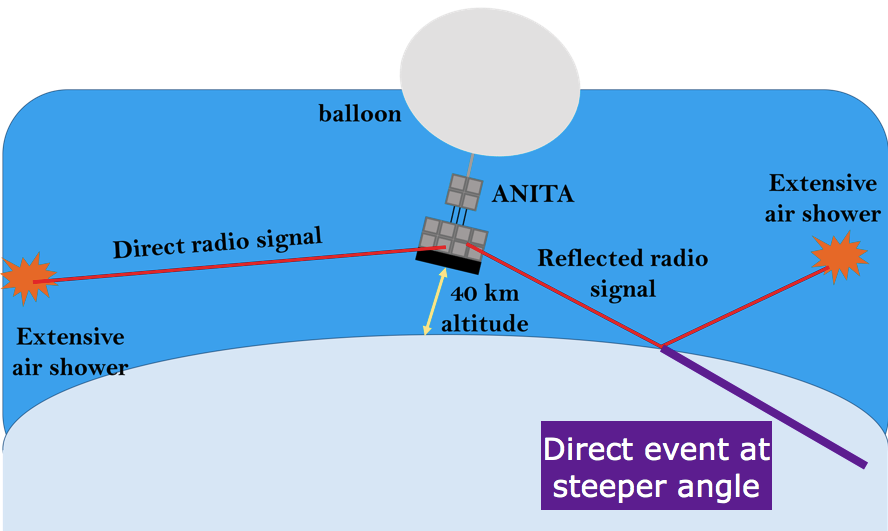
\includegraphics[height=50mm]{anita_cartoon_me.png}
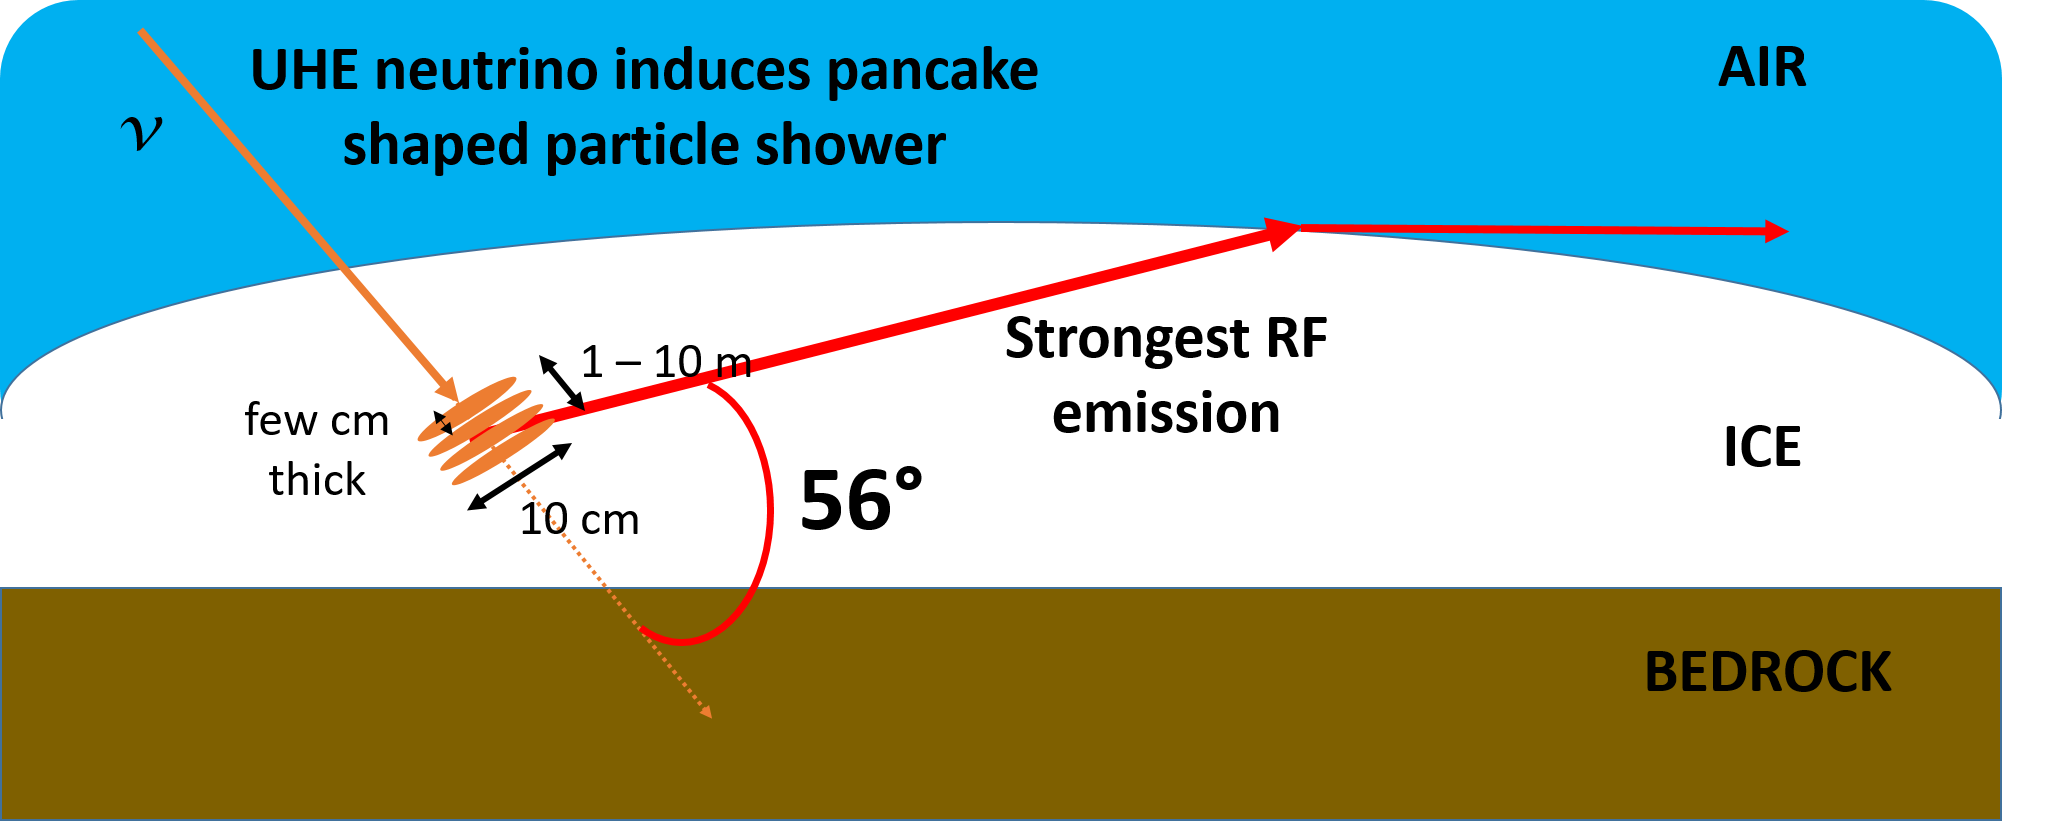
\includegraphics[width=90mm]{askaryan_in_ice.png}
\caption{Left: Cartoon of ANITA looking for radio signals produced by UHE neutrinos interacting in the Antarctic ice. Right: Askaryan effect. }
\label{anita_askaryan}
\end{figure}

\begin{singlespace}
\section{Experimental searches for high energy neutrinos from GRBs}
\end{singlespace}
In this section, we discuss the GRB neutrino searches conducted by the IceCube collaboration in 2012 and 2015, the ANTARES collaboration in 2013, the ANITA collaboration in 2011 and the ARA collaboration in 2015. Since all the mentioned experiments typically conduct diffuse searches, we include a brief overview of how a GRB neutrino search is different from a diffuse search. We also write about the revision of the theoretical prediction for the GRB neutrino flux conducted by Hummer \textit{et al}. in 2012. 

\subsection{GRB neutrino search vs. Diffuse search}
Experiments such as IceCube, ANTARES, ANITA and ARA typically conduct diffuse searches for neutrinos. In diffuse searches, experimenters do not know where neutrinos might be coming from and when. Because experimenters do not know when the signal will arrive in time or direction, to effectively account for backgrounds, thresholds for power and voltage measured must typically be set very high, meaning that experimenters diminish their chance of actually finding a neutrino signal. In setting thresholds high, experiments lose neutrinos. This is an efficiency hit scientists are willing to take to make confident statements about signals they do see. For the GRB neutrino search conducted by each of these experiments, the experimenters knew when and from where neutrinos could be expected. During analysis, for each GRB, scientists had the option to study the data that is temporally close to the expected neutrino events in order to figure out the background for that GRB. From the individual background for each GRB, analysis cuts for each GRB could be determined. In a GRB neutrino search, because the backgrounds can be chosen for smaller time windows and over smaller portions of the sky, analysts can loosen their cuts, and lower thresholds necessary for voltage and power. This typically means GRB neutrino searches have better signal to noise ratio than diffuse neutrino searches because backgrounds can be held lower. 

\subsection{IceCube (2012)}

In 2012, IceCube submitted their first paper on the search for high energy neutrinos from GRBs. They reported an upper limit on the flux of energetic neutrinos associated with GRBs that was at least a factor of $3.7$ below the theoretical predictions and inferred that GRBs were not the only sources of cosmic rays with energies $> 10^{18} \, \mathrm{eV}$ or that the efficiency of neutrino production in GRBs was much lower than had been predicted. See Figure \ref{IC2012money}.\par
They presented results from experiments while the IceCube was still under construction using $40-$ and $59-$string configurations of the detector which took data from April 2008 to May 2009 and from May 2009 to May 2010, respectively. Although the expectation was that neutrinos from pion decay in and around GRBs would arrive at Earth in an equal mixture of flavors, IceCube decided to focus only on searching for muons produced in $\nu_\mu$ ?charged-current interactions \cite{IC2012}. They used observational data for $300$ GRBs with the $40-$ and $59-$string periods of data taking combined. The GRB gamma-emission start ($T_{\mathrm{start}}$) and stop ($T_{\mathrm{stop}}$) times were taken by finding the earliest and latest time reported for gamma-emission.\par
The IceCube collaboration conducted two complementary analyses of the IceCube data: model-dependent and model-independent. In a model-dependent search, data is examined during the period of gamma emission of a GRB for neutrinos with the energy spectrum predicted from the gamma-ray spectra of individual GRBs.
In a model-independent analysis, a more generic search for neutrinos is performed using wider time scales or with different spectra. The model-dependent analysis is more sensitive to emission during the prompt phase of the GRB and more sensitive to harder neutrino emission models. On the other hand, the model-independent analysis is more sensitive to emission on different time scales than the prompt phase and has higher acceptance for lower quality neutrino events. \par
In the $59-$string portion of the model-dependent analysis, no events were found to be both on-source and on time, that is, within $10\degree$ of a GRB \textit{and} between $T_{\mathrm{start}}$ and $T_{\mathrm{stop}}$. In the model-independent analysis, two candidate events were observed, however, subsequent examination showed that they were likely muons from cosmic ray air showers. From the results in \cite{IC2012}, IceCube concluded that theories of cosmic ray and neutrino production in GRBs had to be revisited. 

\begin{figure}[H]
\centering
\includegraphics[width=.6\textwidth]{IC2012money.PNG}
\caption{In this plot, IceCube (2012) showed that the experimental upper bounds to the average neutrino flux and neutrino fluence are lower than the predictions made for the average neutrino flux and neutrino fluence by the analytical model of Guetta \textit{et al.} (2004) \cite{guetta}. From this, they concluded that theories of cosmic ray and neutrino production in GRBs had to be revisited\cite{IC2012}.}
\label{IC2012money}
\end{figure}


\subsection{Revised GRB neutrino flux (2012)}

Following the tension that had arisen between theory and observation, a revision of the neutrino flux from GRBs was conducted in \cite{Hummer} by Hummer \textit{et al}. In 2012, IceCube had used a simplified form of the fireball analytical model by Guetta \textit{et al}. \cite{guetta} for the neutrino flux prediction. This model assumed, for example, that only neutrons could escape the GRB source to contribute to the cosmic ray flux from GRBs. This means that protons stay trapped in the source and produce more neutrinos than in a model where protons can also escape as cosmic rays.\par
In \cite{Hummer}, the neutrino flux was recalculated using numerical methods and following the astrophysical assumptions of the fireball analytical model proposed by Waxman-Bahcall \cite{firstcalc}. The Waxman-Bahcall model does allow protons to escape the source as cosmic rays. Furthermore, additional neutrino production channels, as opposed to only through the $\Delta^{+}$, were considered in this recalculation. Another problem in the analysis of IceCube in 2012 was that they assumed synchrotron losses of pions and muons (decay product of pion) at the same energy but this is not accurate as these two different particles have different masses. This, too, was corrected in \cite{Hummer}. Lastly, the analytical method used by IceCube in 2012 was largely monochromatic, in other words, protons were assumed to interact with photons of only the peak energy. In the revision of \cite{Hummer}, protons were allowed to interact with the whole photon spectrum.\par
A full numerical software package called Neutrinos from Cosmic Accelerators (NeuCosmA) was developed by the authors of \cite{MBthesis,Hummer}. NeuCosmA performs detailed and fast computation of neutrino production in photohadronic $p \gamma$ interactions, via  $\Delta-$resonance, higher resonances (including $K^+$), multi-pion processes, and direct production modes within the Standard Model. It includes energy-loss processes of the secondaries and neutrino flavor oscillations. It takes into account the full spectrum of the photons as opposed to only the spectrum at its peak.\par
Using the same GRB source catalog that IceCube used in 2012, it was found by the developers of NeuCosmA that the total predicted neutrino flux was still about an order of magnitude below IceCube's sensitivity. This careful analysis showed that IceCube's (2012) conclusions were drawn too hastily, and the widely established fireball paradigm of GRB neutrino production had not been probed yet.
 
\subsection{ANTARES (2013)}

In 2013, the ANTARES collaboration published their results from data taken from late 2007 to 2011 using a selected sample of $296$ GRBs \cite{antares}. See Figure \ref{antaresresult}. The parameters needed for the search and the simulation of expected neutrino fluxes were primarily obtained from different GRB catalogs provided by Swift and Fermi. The catalogs were completed using a table supplied by the IceCube collaboration. If a parameter (such as redshift) could not be measured, standard values were used to calculate the spectra. The collaboration excluded bursts for which neither spectral nor fluence information was available. Short GRBs were also discarded as these are much less understood. They also required that the GRBs be located below the local horizon for ANTARES and that the detector was taking reliable physics data during the burst \cite{antares}. \par
For their calculation of the predicted neutrino flux, they used NeuCosmA (see previous subsection). For each GRB, signal neutrino events according to the expected NeuCosmA fluxes were simulated with high statistics and then reconstructed in order to compute the detector's acceptance and the spread of events around the actual burst directions. This distribution yielded the signal probability density function (PDF) $S(\delta)$, where $\delta$ represented the space angle between the reconstructed event direction and the GRB's coordinates. The background PDF $B(\delta)$ was considered to be flat within a $10\degree$ search cone around each burst position. In order to estimate the expected mean number of background events for each burst as realistically as possible, real reconstructed data events were used. For rare events, large time periods are needed to yield enough statistics, which in turn requires averaging over different detector conditions. To compensate, experimenters first estimated the average reconstructed event rate in the GRB's direction using data from the whole late-2007 to 2011 period, and then adjusted for varying detector conditions. The reconstruction algorithm returns a parameter $\Lambda$. A cut on this parameter was used to select well-reconstructed events and to optimize the analysis. Both $S(\delta)$ and $B(\delta)$ depended on the final choice of the cut on $\Lambda$. \par
To summarize, the ANTARES collaboration was the first to present an analysis on detection of high energy neutrinos from GRBs that relied on up-to-date numerical simulations of neutrino emission from GRBs. A search for neutrino events in coincidence with and $10\degree$ around each GRB was conducted. In total, $0.06$ signal events were predicted by NeuCosmA against a background of $0.05$ events. Consistent with this theoretical prediction, no neutrino signal was observed and 90\% confidence upper limits on the fluxes were placed. 
 
\begin{figure}[H]
\centering
\includegraphics[width=.6\textwidth]{antaresresult.PNG}
\caption{Solid lines: sum of the 296 individual gamma-ray burst neutrino spectra used in the ANTARES analysis \cite{antares}, for the analytical model \cite{guetta} in blue and the NeuCosmA model \cite{Hummer, MBthesis} in red. Dashed lines show the ANTARES limits on these fluxes. The IceCube IC40+59 limit \cite{IC2012} on the neutrino emission from 300 GRBs and the first ANTARES limit from its construction phase in 2007 using 40 GRBs are also shown in black (dashed) and grey (dash-dotted), respectively \cite{antares}.}
\label{antaresresult}
\end{figure}

\subsection{IceCube (2015)}
In 2015, IceCube presented updated constraints of the GRB neutrino flux in \cite{IC2015}. This time they used four years of IceCube data and found a single neutrino that was compatible with the atmospheric neutrino background in coincidence with one of the $506$ observed bursts. The neutron model \cite{ahlers}, a scenario where only neutrons escape from the GRB fireball to contribute to the ultra-high energy cosmic ray (UHECR) flux, was now ruled out by this IceCube limit. The model followed by Waxman-Bahcall in \cite{firstcalc,WBub,afterglows,ubrobust} does allow some protons to escape the fireball as UHECRs directly without producing neutrinos. So, this model was not yet ruled out by the IceCube observations. See Figure \ref{IC2015}. 

\begin{figure}[H]
\centering
\includegraphics[width=.6\textwidth]{IC2015.PNG}
\caption{IceCube (2015) finally ruled out the neutron model by Ahlers \textit{et al}. \cite{ahlers} but not the model by Waxman-Bahcall \cite{firstcalc} that allows protons to escape the fireball \cite{IC2015}.}
\label{IC2015}
\end{figure}

\subsection{ANITA (2011)}

In 2011, ANITA set the first limits on the UHE neutrino fluence at energies greater than $10^{18} \, \mathrm{eV}$ from GRBs \cite{anita}. The second flight of the ANITA experiment launched on 2008 December 21, flew for 31 days, 28.5 of which were live days, and recorded over 26 million triggers. Over 98.5\% of the recorded events were fluctuations of thermal noise. ANITA is most sensitive to neutrinos which come from between the horizon and a payload elevation angle (angle above the horizontal) of $-25\degree$ \cite{anita}. There are two ways (geometries) that ANITA can view the radio emission from a neutrino interacting in the ice: \textbf{direct} and \textbf{reflected}. The direct observation occurs when ANITA observes the radio impulse directly from the interaction of an upgoing neutrino. The reflected observation occurs when ANITA receives the radio impulse reflected off of the bottom of an ice shelf (sea water interface) from the interactions of a downgoing neutrino. Since UHE neutrinos are absorbed as they travel through the Earth, most of ANITA's direct events would be associated with neutrinos that \textbf{skim} across the ice. \par
During the 31 day flight of ANITA 2, 26 GRBs were recorded by Swift or Fermi. Of these, only 12 occurred during quiet detection periods while the remaining 14 had significant anthropogenic noise associated with them. ANITA looked for both prompt (any events during the time over which 90\% of the gamma-rays were detected) as well as precursor (any events in the 100 seconds before the start of a burst) neutrinos.\par
The ANITA collaboration performed a so-called blind analysis for their GRB-coincident neutrino search. They set all analysis cuts on regions of time which should contain no neutrino events, and then applied the same cuts in the prompt and precursor emission windows for each burst. To set the analysis cuts, the background period was chosen to be the 55 minutes starting 1 hour before each burst and the 55 minutes starting 5 minutes after each burst (for a total of 1 hour and 50 minutes). This allowed them to use events close to the signal region in time as a background sample without ruling out the possibility of extended prompt or precursor neutrino emission. During the analysis period of setting the cuts, the analysts were blinded to the 10 minutes of signal region having possible neutrino events, hence, the term blind analysis. The blinding makes sure that the analyst's biases on seeing the signal region do not affect the process of setting the cuts.\par
ANITA found no events in the prompt emission or the precursor windows of the observed bursts. This was consistent with the background expectation. They proceeded to set a limit for each burst individually on the prompt UHE neutrino fluence using a Feldman-Cousins 90\% confidence interval, the duration of the burst, and the acceptance calculated using an ANITA Monte Carlo simulation. For each GRB, they configured the Monte Carlo to simulate a point source at the location of the burst, fixed ANITA at the location of the payload during the burst, and assumed an input $E^{-4}$ (for UHE) spectrum. See Figure \ref{anitaresult}.\par
None of the 26 GRBs during the flight had a payload elevation angle between $-25 \degree$ and the horizon which is where ANITA has the best chance of seeing direct neutrino events. Of the 12 GRBs observed during quiet time, the most promising direct observation geometry was from GRB $090113$ at an elevation angle of $-25.7\degree$ although this still suffered from poor geometry. ANITA placed a 90\% confidence level limit on the $E^{-4}$ prompt neutrino fluence for energies $10^{17} \, \mathrm{eV} < E < 10^{21} \, \mathrm{eV}$ of $E^{4} \, \Phi = 1.5 \times 10^{20} \, \mathrm{ GeV^{3} \, cm^{-2}}$ from GRB $090113$. 

\begin{figure}[H]
\centering
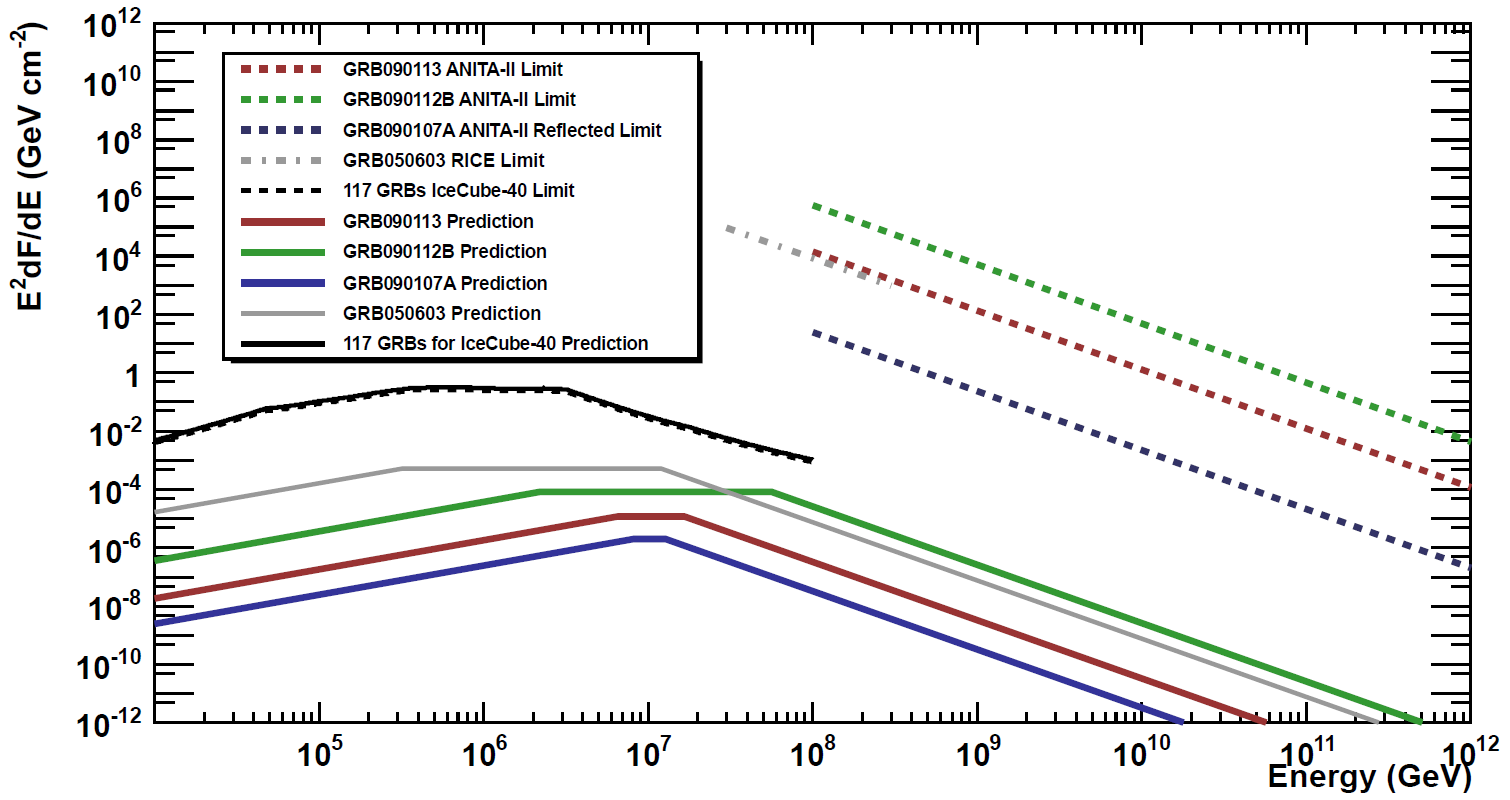
\includegraphics[width=.6\textwidth]{anitaresult.PNG}
\caption{The two best direct limits by ANITA on the UHE neutrino fluence from the blind analysis are from GRB 090113 and GRB 090112B. These are shown with red and green dashed lines respectively. The best reflected limit is from GRB 090107A, shown with a blue dashed line. RICE (Besson \textit{et al}. 2007) and IceCube (2012) \cite{IC2012} limits are also shown. The IceCube limit is an aggregate limit based on 117 individual GRBs, and is based on a fluence prediction from Guetta \textit{et al}. (2004) \cite{guetta,anita}.}
\label{anitaresult}
\end{figure}


\subsection{ARA (2015)}

In 2015, the ARA collaboration presented an UHE GRB neutrino fluence limit from 57 selected GRBs and the first limit on the UHE GRB quasi-diffuse neutrino flux for energies $10^{16} \, \mathrm{ eV}$ to $10^{19} \, \mathrm{ eV}$ \cite{araproto} using data collected by ARA in prototype form (ARA Testbed) \cite{arahardware}. See Figure \ref{arafluence} and Figure \ref{araquasiflux}. \par
The quasi-diffuse flux is an estimation of the average GRB flux calculated from a statistically representative set of GRBs and is useful in comparing limits between experiments that observe different sets of bursts. \par
Predictions for GRB neutrino fluences were calculated using NeuCosmA. For all GRBs, the bulk Lorentz factor of the fireball $\Gamma$ was assumed to be 316 and the baryonic loading (ratio of fractional proton energy to fractional electron energy) was assumed to be 10. As ARA is sensitive to all neutrino flavors, neutrino fluence predictions for all three flavors were obtained from NeuCosmA with 1:1:1 flavor ratio assumption. AraSim, a Monte-Carlo simulation software package used within the ARA collaboration, was used to simulate neutrino signals as they would be observed by the detector. It simulates the full chain of neutrino events such as the neutrino's path through the Earth, radio Cherenkov emission, the path and response of the emitted signal in the ice, and the trigger and data acquisition mechanisms of the detector \cite{araproto}. 
\par
Among 589 GRBs monitored by the Gamma Ray Coordinate Network (GCN) catalog from January 2011 to December 2012 over the entire sky, 57 GRBs were selected for analysis because they occurred during a period of low anthropogenic background and high stability of the station and fell within the geometric acceptance. \par
Drawing on the blinding technique of analysis carried out by the ANITA GRB neutrino search, the ARA collaboration performed a blind analysis with two un-blinding steps. ARA, too, used the 55 minutes before 1 hour and the 55 minutes after 5 minutes of a burst to study the background for each burst. For an extra step of caution, initially, only 10\% of the total 110 minutes of data temporally close to the 10 minutes of signal region was used to get cuts. Then, the remaining 90\% was used to get cuts and it was checked that these cuts were consistent with the ones from the initial 10\%. Only after this two-step method of getting analysis cuts was the analyzer unblinded to the signal region. \par
In the search for UHE neutrinos from 57 GRBs in \cite{araproto}, 0 events were observed, which was consistent with 0.11 expected background events.


\begin{figure}[H]
\centering
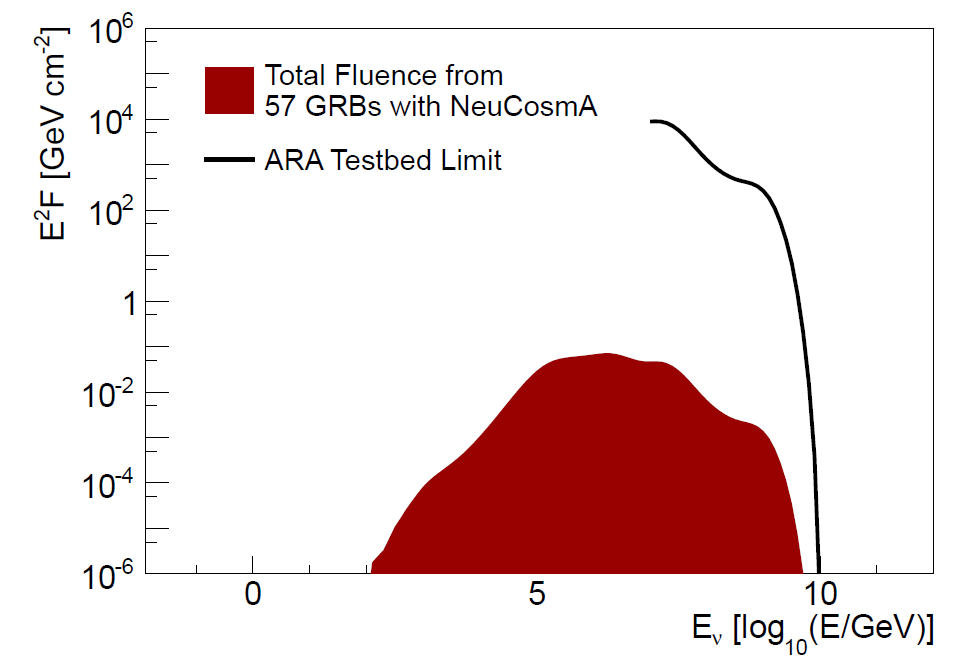
\includegraphics[width=.532\textwidth]{ara_limit.png}
\caption{The limit on the UHE GRB neutrino fluence from 57 GRBs used for ARA analysis. Total fluence from NeuCosmA for the 57 GRBs is shown with a red shaded area and the limit from the ARA Testbed above $10^{16}$ eV is shown with a black solid curve \cite{araproto}.}
\label{arafluence}
%\end{figure}
%\begin{figure}[H]
\centering
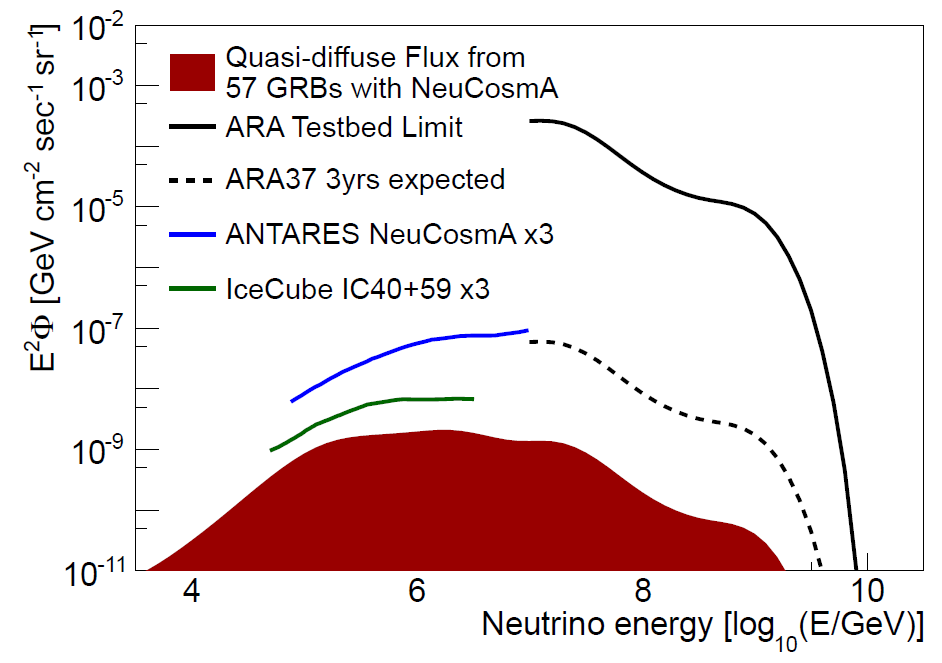
\includegraphics[width=.532\textwidth]{ara_quasi_diffuse_limits.png}
\caption{The inferred quasi-diffuse all flavor flux limit from the selected 57 GRBs. IceCube and ANTARES limits are from \cite{IC2012} and \cite{antaresmuon}, respectively. In 2015, IceCube published a search for neutrinos from GRBs based on four years of data \cite{IC2015}, but that paper did not include a limit on the quasi-diffuse flux. Preliminary estimates indicate that the latest result would improve upon the IC40+59 limit \cite{IC2012} shown here by about an order of magnitude. Since the published limits for both IceCube and ANTARES are based on a muon neutrino flux, an additional factor of three has been applied in \cite{araproto} on this plot in order to account for all three neutrino flavors. The ARA37 expected limit is the trigger level sensitivity based on the diffuse neutrino search \cite{araprotofirst}.}
\label{araquasiflux}
\end{figure}


%------------------------------------------------------------------------
%-----------------------NEW SECTION----------------------------
%------------------------------------------------------------------------
\begin{singlespace}
\section{Prospects for detection of high energy neutrinos from GRBs}
\end{singlespace}
So far, no high energy neutrinos from GRBs have been observed, and this observation is not inconsistent with revised theoretical predictions. Experiments have only started to conduct GRB neutrino searches and in a few years, experiments such as IceCube, ANTARES and ARA will have had time to collect more data that is in coincidence with observed GRBs. There are around 600 potentially observable GRBs per year. So when these experiments do a neutrino search for data collected over multiple years, the number of GRBs coinciding with their data increases. It is more likely that an analysis of data in coincidence with 500 GRBs will yield a neutrino signal as opposed to an analysis of data in coincidence with only 50. \par 
Experiments such as IceCube are also becoming increasingly sensitive to neutrinos predicted to accompany the prompt emission of a GRB. In \cite{IC2pev}, the IceCube collaboration presented a paper on the first evidence for a high energy neutrino flux of extraterrestrial origin. Using data from 2010-2013, they reported an astrophysical neutrino flux in the $100 \, \mathrm{TeV - PeV}$ range at the level of $10^{-8} \, \mathrm{GeV \, cm^{-2} \,  s^{-1} \,  sr^{-1}}$ per flavor and rejected a purely atmospheric explanation for the combined 3-year data at $5.7\sigma$. They concluded that the data was consistent with expectations for equal fluxes of all three neutrino flavors and with isotropic arrival directions, suggesting either numerous or spatially extended sources. The three-year data set, with a livetime of 988 days, contained a total of 37 neutrino candidate events with deposited energies ranging from 30 to $2000 \, \mathrm{TeV}$. The $2000 \, \mathrm{TeV}$ or $2 \, \mathrm{PeV}$ event is the highest-energy neutrino interaction ever observed. Since the prompt emission GRB neutrino peak is at $\sim 0.1-1 \, \mathrm{PeV}$ and IceCube can detect order of PeV neutrinos, we conclude that IceCube has the potential to observe GRB prompt emission neutrinos. Observation of GRB prompt emission neutrinos of order of PeV by IceCube would be unambiguous proof of hadronic acceleration in GRBs and could also explain the origin of UHE cosmic rays.  
 \par
KM3NeT, described in \cite{km3net}, is a deep-sea neutrino telescope being constructed in the Mediterranean Sea. It is building upon the concepts of neutrino detection followed by the ANTARES collaboration. It will host the next generation Cherenkov neutrino telescope and complement IceCube in its field of view and potentially exceed it substantially in sensitivity. The main goal of this telescope is to detect high energy neutrinos of astrophysical origin which includes GRB neutrinos.\par
The KM3NeT collaboration has plans to focus on detection of high energy neutrinos from galactic sources such as the supernova remnant RXJ1713.7-3946 and the pulsar wind nebula Vela X. Gamma-rays in the TeV region have been measured for these sources. Assuming an exponential cut-off power law for the neutrino energy spectrum and simulating different solutions for the detector design, the conclusion is that with the planned detector arrangement, KM3NeT can claim a discovery after about 5 years of observation and the observation at a significant level of $3\sigma$ with 50\% confidence limit after 2 years, for RXJ1713.7-3946. A shorter observation time (about 3 years for the discovery and slightly more than 1 year for the observation) would be necessary in the case of Vela X \cite{km3net}. Thus, KM3NeT, too, holds the potential to detect high energy neutrinos that are predicted to accompany the prompt emission of a GRB which would provide evidence for hadronic acceleration in GRBs. 
\par
On the UHE side of the story, ANITA is naturally limited in that it observes for only about a month when launched and, therefore, has to perform its analysis with a much smaller set of GRBs. However, it was concluded in \cite{anita} that there is room for about a factor of 5 improvement with ANITA 3 if a GRB occurs with a good geometry relative to the payload. ANITA 3 has flown already and its data is still being analyzed. The ANITA collaboration is preparing to launch ANITA 4 in 2016 with improved hardware, waveform sampling and triggering techniques.\par
The ARA collaboration is preparing for deployment of at least 3 more of its deep stations in 2017. It was concluded in \cite{araproto} that future analyses from two ARA deep stations (200 m deep) should have at least a factor of 6 improvement in sensitivity compared to the analysis with the ARA Testbed.\par
ANITA and especially, ARA, have the potential to observe GRB neutrinos of the UHE regime. UHE neutrinos have been predicted to accompany the afterglow emission of GRBs in the fireball model. The afterglow emission is thought to come from collisions of the fireball ejecta with its surrounding medium. This could be tested with observations of UHE neutrinos by ANITA and ARA.\par
If any of the above mentioned experiments were to observe high energy neutrinos correlated with GRBs, the fireball paradigm of GRBs could be probed. For example, if a neutrino of energy of order 100 TeV correlated with a GRB is observed to accompany the prompt emission of that GRB, by IceCube, ANTARES or KM3NeT, that would confirm predictions made by the fireball model in \cite{firstcalc}. If neutrinos of significantly lower energies are seen instead during prompt emission, that would help to constrain the fireball model. Similarly if UHE neutrinos are seen instead during prompt emission by ANITA or ARA, one might conclude that hadrons are accelerated to even greater energies in the fireball than initially predicted. Thus observation of neutrinos in the different energy regimes by these different experiments can provide constraints on the fireball model of GRBs.\par
We conclude that neutrino telescopes have only barely started to probe the fireball paradigm of GRB neutrino production and a lot remains to be discovered by future searches. The experiments we discuss in this paper cover different regions of the energy spectrum and so future searches might be able to constrain different parts of the fireball model. Some of them such as ARA and KM3NeT are still being built and have not reached their complete potential yet. Others such as IceCube and ANITA are undergoing upgrades. Thus, we are optimistic that as these experiments conduct future searches we will learn more about the physics of GRBs from the results we obtain in different energy regimes. 
 
%------------------------------------------------------------------------
%-----------------------NEW SECTION----------------------------
%------------------------------------------------------------------------
\section{Acknowledgments}
I would like to thank my advisor Prof. Amy Connolly and her research group here at OSU. I am very grateful for the opportunity to be a part of the Connolly group efforts towards ultra-high energy neutrino detection with the ANITA and ARA experiments. I thank Prof. Connolly for always being there for me with her excellent advising and mentorship. In the Connolly group, I give special thanks to graduate student Brian Clark and postdoctoral researcher Carl Pfendner for their invaluable guidance and help with my candidacy work. I thank CCAPP postdoctoral fellow Mauricio Bustamante for his explanation of different concepts of GRB theory and help with finding useful references on the topic. Lastly, I thank the Physics and Astronomy departments of OSU for supporting me through a graduate teaching associateship during the period of my candidacy work. 
\end{doublespace}

\newpage
\bibliographystyle{unsrt}
\refstepcounter{section}
\bibliography{references}


\end{document}


